\documentclass[12pt,a4paper,ngerman]{article}
\usepackage{stylesheet}
\usepackage{epstopdf}
\begin{document}

\TUHeader                          %  Bitte Ausfüllen!!!
%----------------------------
{Übung F: Übertragungsverhalten nachrichtentechnischer Systeme}                       %  Übungstitel
%----------------------------
{25.11.2014}                        %  Übungsdatum
%----------------------------
{05}                            %  Gruppen-Nr.
%----------------------------
{Thomas Neff}                   % Name des Protokollführers
%----------------------------
{
1.~Daniel Freßl, 1230028\\
2.~Thomas Neff, 1230319\\                    %  Übungsteilnehmer
3.~Thomas Pichler, 1230320 \\                   %  ...bei <4 Teilnehmer auskommentieren
4.~Martin Winter, 1130688\\
5.~Bernadette Schreyer, 1073076\\
}
%----------------------------
{Ao.Univ.-Prof. Dipl.-Ing. Dr. techn. Erich Leitgeb}
{Max Henkel}                          %  Betreuer
%----------------------------
{Graz}                              %  Ort der Protokollerstellung
{\today}                            %  Datum Protokollerstellung




\pagebreak
  
\tableofcontents
  
\pagebreak

%-------------------------------------------------------------------------------
%
% Beginn des Protokolls
%
%-------------------------------------------------------------------------------

\section{Rückwirkungsfreie Messung des H-Feldes zweier PCD-Schleifenantennen mit unterschiedlichen Güten}
\subsection{Aufgabenstellung}
Bei dieser Aufgabe sollten zwei Antennen mit unterschiedlicher Güte (5, 50) miteinander verglichen werden. Dazu soll die magnetische Feldstärke in Abhängigkeit von der Entfernung zur Antenne gemessen werden (in 5mm Schritten, von 0 bis 14cm).\\
Weiters soll die Anstiegszeit des Sendesignals, von 10\% auf 90\% der Trägersignalamplitude, für beide Antennen bestimmt werden.

\subsection{Messaufbau}
Für den Messaufbau wurde ein speziell dafür modifizierter RFID-Reader mit regelbarer Ausgangsamplitude verwendet. Dieser wurde an einen Computer und einen Verstärker angeschlossen. Zwischen Verstärker und zu vermessender Antenne wurde ein Dämpfer (6db) eingebaut.\\
Die Antenne und die zur Messung verwendete Referenzspule wurden in einen verstellbaren Distanzhalter platziert. Zur Messung wurde die Referenzspule an ein Oszilloskop angeschlossen.

\subsection{Tabellen}
\begin{table}[H]
\begin{center}
\begin{tabular}{ |c|c|c|c|c| }
  \hline
     & Q=50 & Q=5 & Q=50 & Q=5\\

    Distanz & $U_i(pp)$ & $U_i(pp)$ & H(rms) & H(rms)\\

  [cm] & [V] & [V] & [A/m] & [A/m] \\
  \hline
  0 & $2.9$ & $0.894$ & $3.167$ & $0.976$ \\
  \hline
  $0.5$ & $2.75$ & $0.863$ & $3.003$ & $0.942$ \\
  \hline
  $1$ & $2.61$ & $0.813$ & $2.85$ & $0.888$ \\
  \hline
  $1.5$ & $2.44$ & $0.756$ & $2.664$ & $0.826$ \\
    \hline
  $2$ & $2.25$ & $0.706$ & $2.457$ & $0.771$ \\
    \hline
  $2.5$ & $2.06$ & $0.637$ & $2.249$ & $0.696$ \\
    \hline
  $3$ & $1.89$ & $0.584$ & $2.064$ & $0.638$ \\
    \hline
  $3.5$ & $1.7$ & $0.531$ & $1.86$ & $0.579$\\
    \hline
  $4$ & $1.55$ & $0.481$ & $1.69$ & $0.525$ \\
    \hline
  $4.5$ & $1.39$ & $0.434$ & $1.52$ & $0.474$ \\
    \hline
  $5$ & $1.25$ & $0.425$ & $1.37$ & $0.464$ \\
    \hline
  $5.5$ & $1.13$ & $0.425$ & $1.23$ & $0.464$ \\
     \hline
  $6$ & $1.01$ & $0.425$ & $1.102$ & $0.464$ \\
      \hline
  $6.5$ & $0.92$ & $0.425$ & $1.004$ & $0.464$ \\ 
      \hline
  $7$ & $0.82$ & $0.425$ & $0.895$ & $0.464$ \\
      \hline
  $7.5$ & $0.75$ & $0.425$ & $0.819$ & $0.464$ \\
      \hline
  $8$ & $0.68$ & $0.425$ & $0.743$ & $0.464$ \\
      \hline
  $8.5$ & $0.62$ & $0.425$ & $0.677$ & $0.464$ \\
      \hline
  $9$ & $0.55$ & $0.425$ & $0.6$ & $0.464$ \\
      \hline
  $9.5$ & $0.5$ & $0.425$ & $0.546$ & $0.464$ \\
      \hline
  $10$ & $0.46$ & $0.425$ & $0.502$ & $0.464$ \\
      \hline
  $10.5$ & $0.41$ & $0.425$ & $0.448$ & $0.464$ \\
      \hline
  $11$ & $0.38$ & $0.425$ & $0.415$ & $0.464$ \\
      \hline
  $11.5$ & $0.35$ & $0.425$ & $0.382$ & $0.464$ \\
      \hline
  $12$ & $0.32$ & $0.425$ & $0.349$ & $0.464$ \\
      \hline
  $12.5$ & $0.29$ & $0.425$ & $0.317$ & $0.464$ \\
      \hline
  $13$ & $0.29$ & $0.425$ & $0.317$ & $0.464$ \\
      \hline
  $13.5$ & $0.29$ & $0.425$ & $0.317$ & $0.464$ \\
        \hline
  $14$ & $0.29$ & $0.425$ & $0.317$ & $0.464$ \\  \hline
\end{tabular}
\caption{Gemessene Spannung bei verschiedenen Höhen und Güten}
\end{center}
\label{tab:1}
\end{table}
\pagebreak
\subsection{Formeln}
Diese Formel stellt den Zusammenhang zwischen induzierter Spannung und Feldstärke dar. Die verwendeten Parameter sind $f_r = 13.56$MHz, $\mu_0 = 4\pi \cdot 10^{-7}\frac{As}{Vm}$, $\mu_r = 1$ und $A = 0.072 \cdot 0.042\ m^2$.
\begin{equation}
U_{ind} = 2\pi \cdot f_r \cdot \mu_0 \cdot \mu_r \cdot H \cdot A
\end{equation}

Zusammenhang zwischen Spitze-Spitze-Spannung und dem Effektivwert der Spannung.
\begin{equation}
U_{pp} = \sqrt{2}  \cdot 2 \cdot U_{ind}
\end{equation}

\subsection{Berechnungsbeispiele}
Die Werte für das Berechnungsbeispiel wurden aus der Tabelle \ref{tab:1} Zeile 1 entnommen.
\begin{equation}
U_{ind} = \frac{U_{pp}}{\sqrt{2}  \cdot 2} = \frac{2.9V}{\sqrt{2}  \cdot 2} = 1.025V
\end{equation}

\begin{gather}
H = \frac{U_{ind}}{2\pi \cdot f_r \cdot \mu_e \cdot \mu_r \cdot A} = \\
\frac{1.025V}{2\pi \cdot 13.56MHz \cdot 4\pi \cdot 10^{-7}\frac{As}{Vm} \cdot 1 \cdot 0.072m \cdot 0.042m} = 3.167\frac{A}{m}
\end{gather}

\subsection{Diagramme}
\begin{figure}[H]
\centering
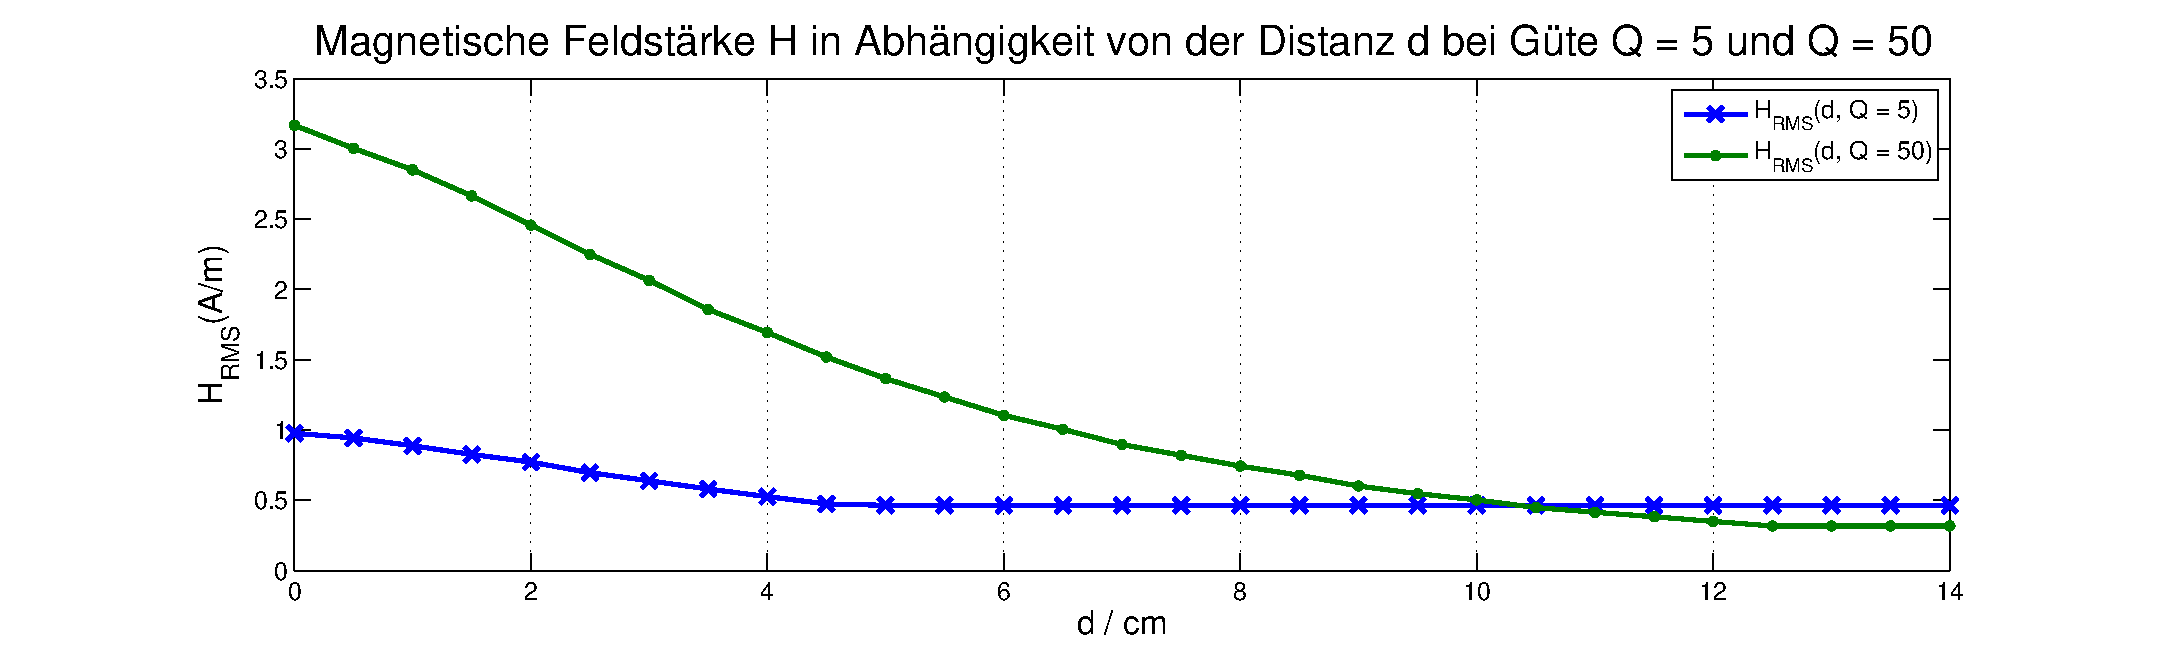
\includegraphics[width=1.1\textwidth]{figures/a1.eps} 
\caption{Verlauf der Feldstärke über die Entfernung für Q = 5 und Q = 50}
\label{fig:1_q5}
\end{figure}

\begin{figure}[H]
\centering
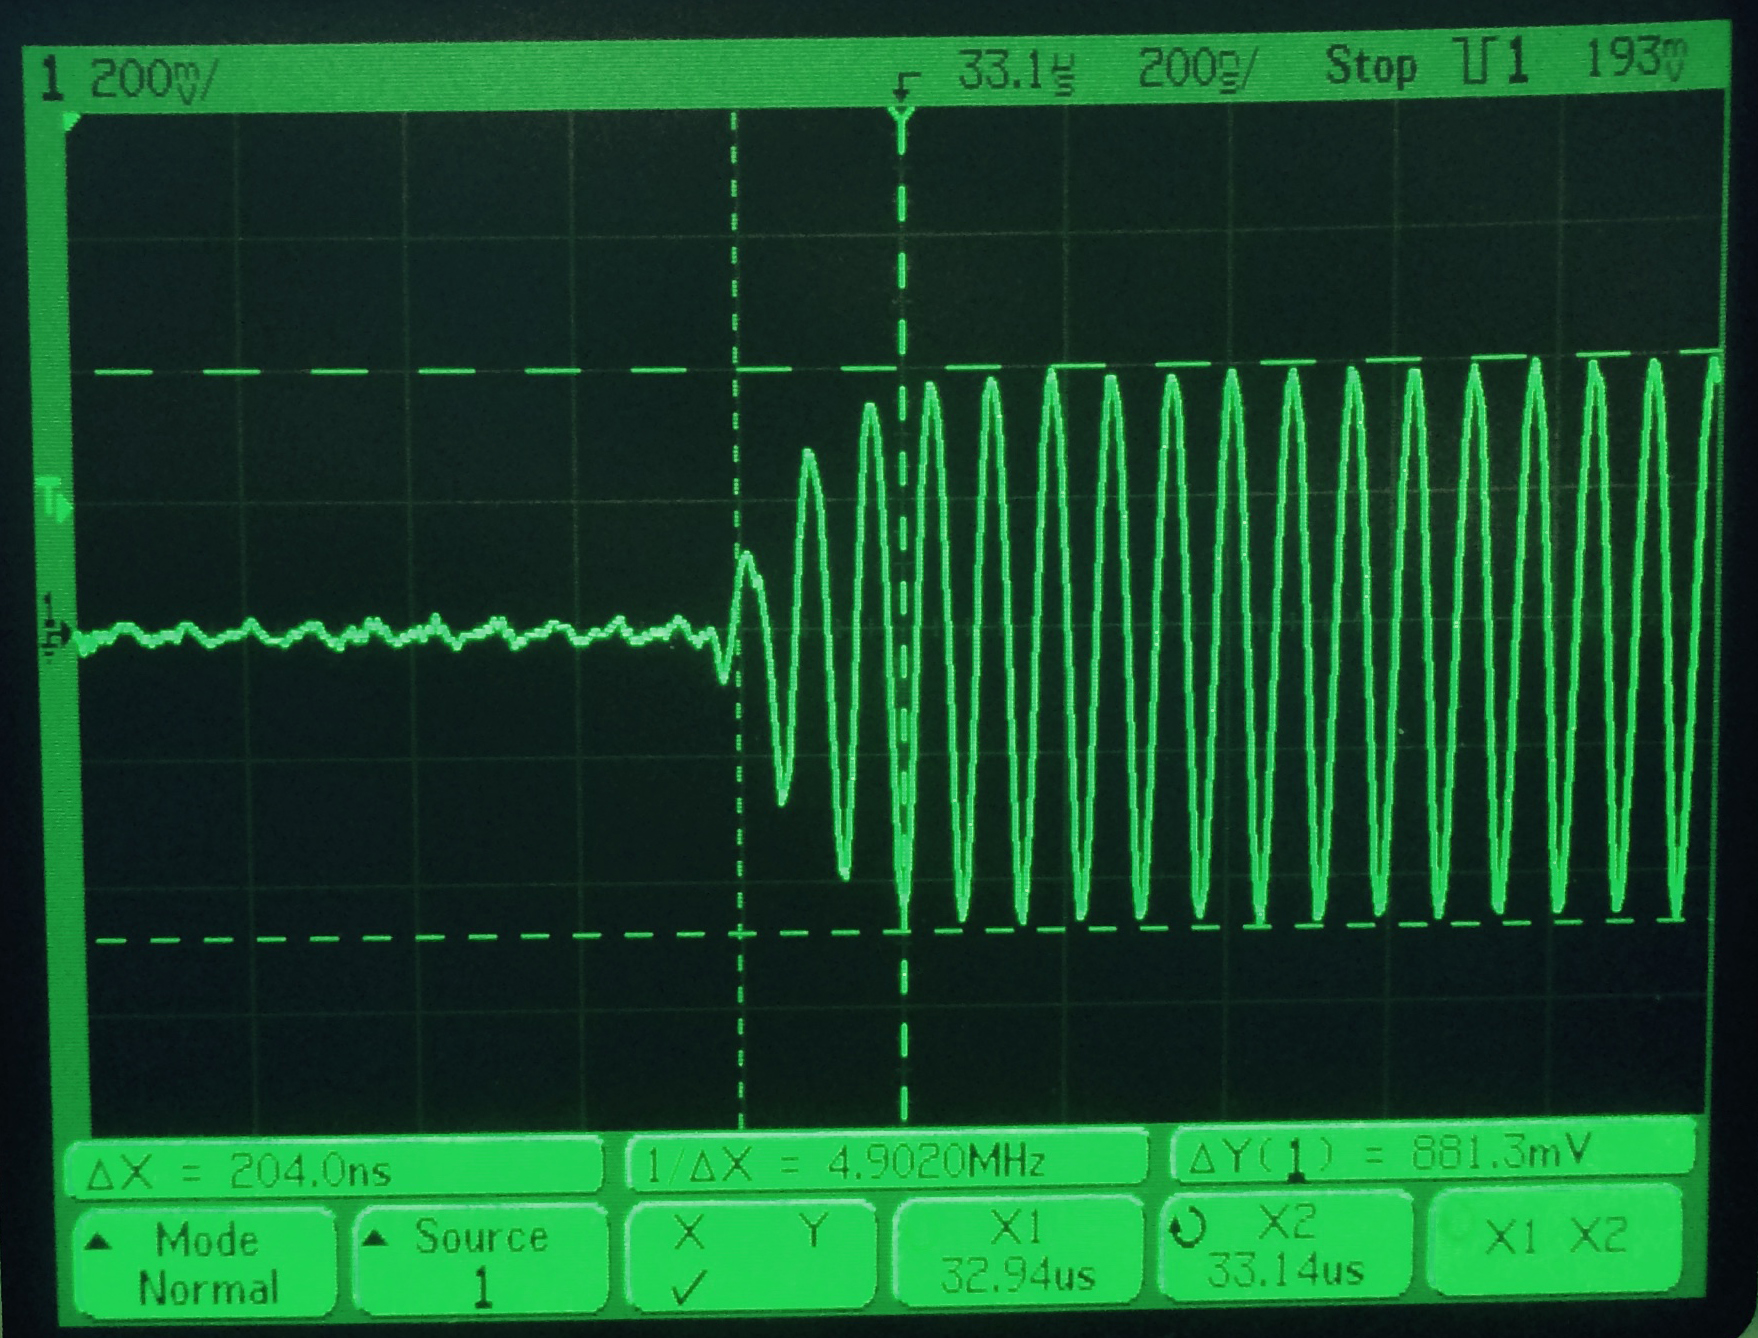
\includegraphics[width=0.9\textwidth]{figures/Anstiegq5.jpg} 
\caption{Messung der Anstiegszeit der Antenne mit Q = 5 am Oszilloskop}
\label{fig:1_anstieg}
\end{figure}

\subsection{Geräteliste}
\begin{itemize}
\item Computer
\item Reader: Labor-RFID-Reader
\item Verstärker: Amplifier Research Model 75A250
\item Dämpfer: 6dB
\item Antennen: PCD-Schleifenantennen mit Q=5 und Q=50
\item Referenzspule mit Abmessungen 72mm x 42mm
\item Oszilloskop: Agilent 54622D
\item Distanzhalter: verstellbar
\end{itemize}
\pagebreak
\subsection{Diskussion}
Bei dieser Übung wurde jeweils eine Antenne (mit der Güte Q=5, Q=50) in den Aufbau eingesetzt und angeschlossen. Es wurde nur das Trägersignal ohne zusätzliche Information übertragen und mit der Referenzspule gemessen. Die Entfernung der Referenzspule zur Antenne wurde mit 5mm Schritten von 0cm auf 14cm verändert. Mit dem Oszilloskop wurde die Peak-Peak-Spannung gemessen.\\
Diese Spannung kann mit den oben angeführten Formeln in die magnetische Feldstärke umgerechnet werden. Bei der Umrechnung ist zu beachten, das die magnetische Feldstärke als Effektivwert angegeben werden soll und die Spannung als Spitze-Spitze-Wert gemessen wird.\\
Die gemessenen und berechneten Werte wurden in einem Diagramm (Abbildung \ref{fig:1_q5}) dargestellt.\\
Die magnetische Feldstärke ist bei der Antenne mit der Güte Q=50 bis zu einer Entfernung von 10cm höher.\\
\\
Zur Messung der Anstiegszeit wurde beim Oszilloskop der Single-Shot-Modus und Triggern an der fallenden Flanke mit nachfolgender Pause von $1.5\mu s$ eingestellt.\\
Der Reader wurde über die Reader-Software am Computer zum Senden eines Lesebefehls veranlasst, welcher an der Referenzspule und somit am Oszilloskop die zum Triggern benötigte negative Flanke und nachfolgende Pulsbreite (Pause) erzeugt.\\
Nach dieser Pause steigt die Amplitude des Signals wieder auf die Amplitude des Trägersignals an. Die Zeit für diesen Anstieg von 10\% auf 90\% der Signalamplitude wurde mittels Marker am Oszilloskop gemessen.\\
\begin{itemize}
\item Antenne Q = 50: $1.24\mu s$
\item Antenne Q = 5:  $204ns$
\end{itemize}
Aus diesen Werten ist ersichtlich, das die Anstiegszeit für höhere Güten größer wird. Somit kann mit Antenne mit höherer Güte zwar eine größere Reichweite aber eine geringere Datenrate erzielt werden.


\pagebreak



\section{Messung der H-Feldstärke über der Frequenz bei unterschiedlichen Antennengüten}
\subsection{Aufgabenstellung}
Bei dieser Aufgabe soll der Frequenzgang beider Antennen (Q = 5, Q = 50) von 12MHz bis 15MHz aufgenommen werden.\\

\subsection{Messaufbau}
Als Signalquelle wurde ein Funktionsgenerator verwendet, dieser wurde über den Verstärker und Dämpfer an die jeweilige Antenne angeschlossen.
Die Antenne wurde mittig in den ISO-Aufbau eingebracht, auf einer Seite (der Helmholtz-Anordnung) wurde die Referenzspule befestigt. 
Die induzierte Spannung an der Referenzspule wurde auf einem Oszilloskop dargestellt. 

\subsection{Tabellen}
\begin{table}[H]
\begin{center}
\begin{tabular}{ |c|c|c|c|c| }
  \hline
     & Q=50 & Q=5 & Q=50 & Q=5\\
    Frequenz & $U_i(pp)$ & $U_i(pp)$ & H(rms) & H(rms)\\

  {[MHz]} & {[V]} & {[V]} & {[A/m]} & {[A/m]} \\
  \hline
  12 & $0.363$ & $0.5$ & $0.4479$ & $0.6170$ \\
  \hline
  $12.2$ & $0.425$ & $0.575$ & $0.5158$ & $0.6979$ \\
  \hline
  $12.4$ & $0.5$ & $0.6$ & $0.5971$ & $0.7165$ \\
  \hline
  $12.6$ & $0.784$ & $0.813$ & $0.9214$ & $0.9554$ \\
    \hline
  $12.8$ & $1$ & $0.844$ & $1.1568$ & $0.9764$ \\
    \hline
  $13$ & $1.3$ & $0.869$ & $1.4808$ & $0.9898$ \\
    \hline
  $13.2$ & $1.78$ & $0.887$ & $1.9968$ & $0.9950$ \\
     \hline
  $13.25$ & $1.97$ & $0.894$ & $2.2016$ & $0.9991$ \\ 
    \hline
  $13.3$ & $2.14$ & $0.9$ & $2.3826$ & $1.0020$ \\
    \hline
  $13.35$ & $2.31$ & $0.906$ & $2.5622$ & $1.0049$ \\
    \hline
  $13.4$ & $2.5$ & $0.906$ & $2.7626$ & $1.0012$ \\
    \hline
  $13.45$ & $2.64$ & $0.906$ & $2.9065$ & $0.9974$ \\
    \hline
  $13.5$ & $2.73$ & $0.913$ & $2.9944$ & $1.0014$ \\
     \hline
  $13.55$ & $2.76$ & $0.913$ & $3.0162$ & $0.9977$ \\
      \hline
  $13.6$ & $2.7$ & $0.913$ & $2.9397$ & $0.9941$ \\ 
      \hline
  $13.65$ & $2.61$ & $0.919$ & $2.8313$ & $0.9969$ \\
      \hline
  $13.7$ & $2.45$ & $0.925$ & $2.6481$ & $0.9998$ \\
      \hline
  $13.75$ & $2.31$ & $0.925$ & $2.4877$ & $0.9961$ \\
      \hline
  $13.8$ & $2.14$ & $0.925$ & $2.2962$ & $0.9925$ \\
      \hline
  $14$ & $1.59$ & $0.925$ & $1.6817$ & $0.9784$ \\
      \hline
  $14.2$ & $1.23$ & $0.925$ & $1.2826$ & $0.9646$ \\
      \hline
  $14.4$ & $1.02$ & $0.919$ & $1.0489$ & $0.9450$ \\
      \hline
  $14.6$ & $0.86$ & $0.906$ & $0.8722$ & $0.9189$ \\
      \hline
  $14.8$ & $0.734$ & $0.9$ & $0.7344$ & $0.9005$ \\
      \hline
  $15$ & $0.653$ & $0.887$ & $0.6446$ & $0.8756$ \\
      \hline
\end{tabular}
\caption{Gemessene Spannung und berechnete Feldstärke über die Frequenz}
\label{tab:2}
\end{center}
\end{table}
\subsection{Formeln}
Diese Formel stellt den Zusammenhang zwischen induzierter Spannung und Feldstärke dar. Die verwendeten Parameter sind $f_r = 13.56$MHz, $\mu_0 = 4\pi \cdot 10^{-7}\frac{As}{Vm}$, $\mu_r = 1$ und $A = 0.072 \cdot 0.042\ m^2$.
\begin{equation}
U_{ind} = 2\pi \cdot f_r \cdot \mu_0 \cdot \mu_r \cdot H \cdot A
\end{equation}

Zusammenhang zwischen Spitze-Spitze-Spannung und dem Effektivwert der Spannung.
\begin{equation}
U_{pp} = \sqrt{2}  \cdot 2 \cdot U_{ind}
\end{equation}
\pagebreak
\subsection{Berechnungsbeispiele}
Die Werte für das Berechnungsbeispiel wurden aus der Tabelle \ref{tab:2} Zeile 1 entnommen.
\begin{equation}
U_{ind} = \frac{U_{pp}}{\sqrt{2}  \cdot 2} = \frac{0.363V}{\sqrt{2}  \cdot 2} = 0.1283 V
\end{equation}

\begin{gather}
H = \frac{U_{ind}}{2\pi \cdot f_r \cdot \mu_e \cdot \mu_r \cdot A} = \\
\frac{0.1283V}{2\pi \cdot 12MHz \cdot 4\pi \cdot 10^{-7}\frac{As}{Vm} \cdot 1 \cdot 0.072m \cdot 0.042m} = 0.448\frac{A}{m}
\end{gather}

\subsection{Diagramme}
\begin{figure}[H]
\centering
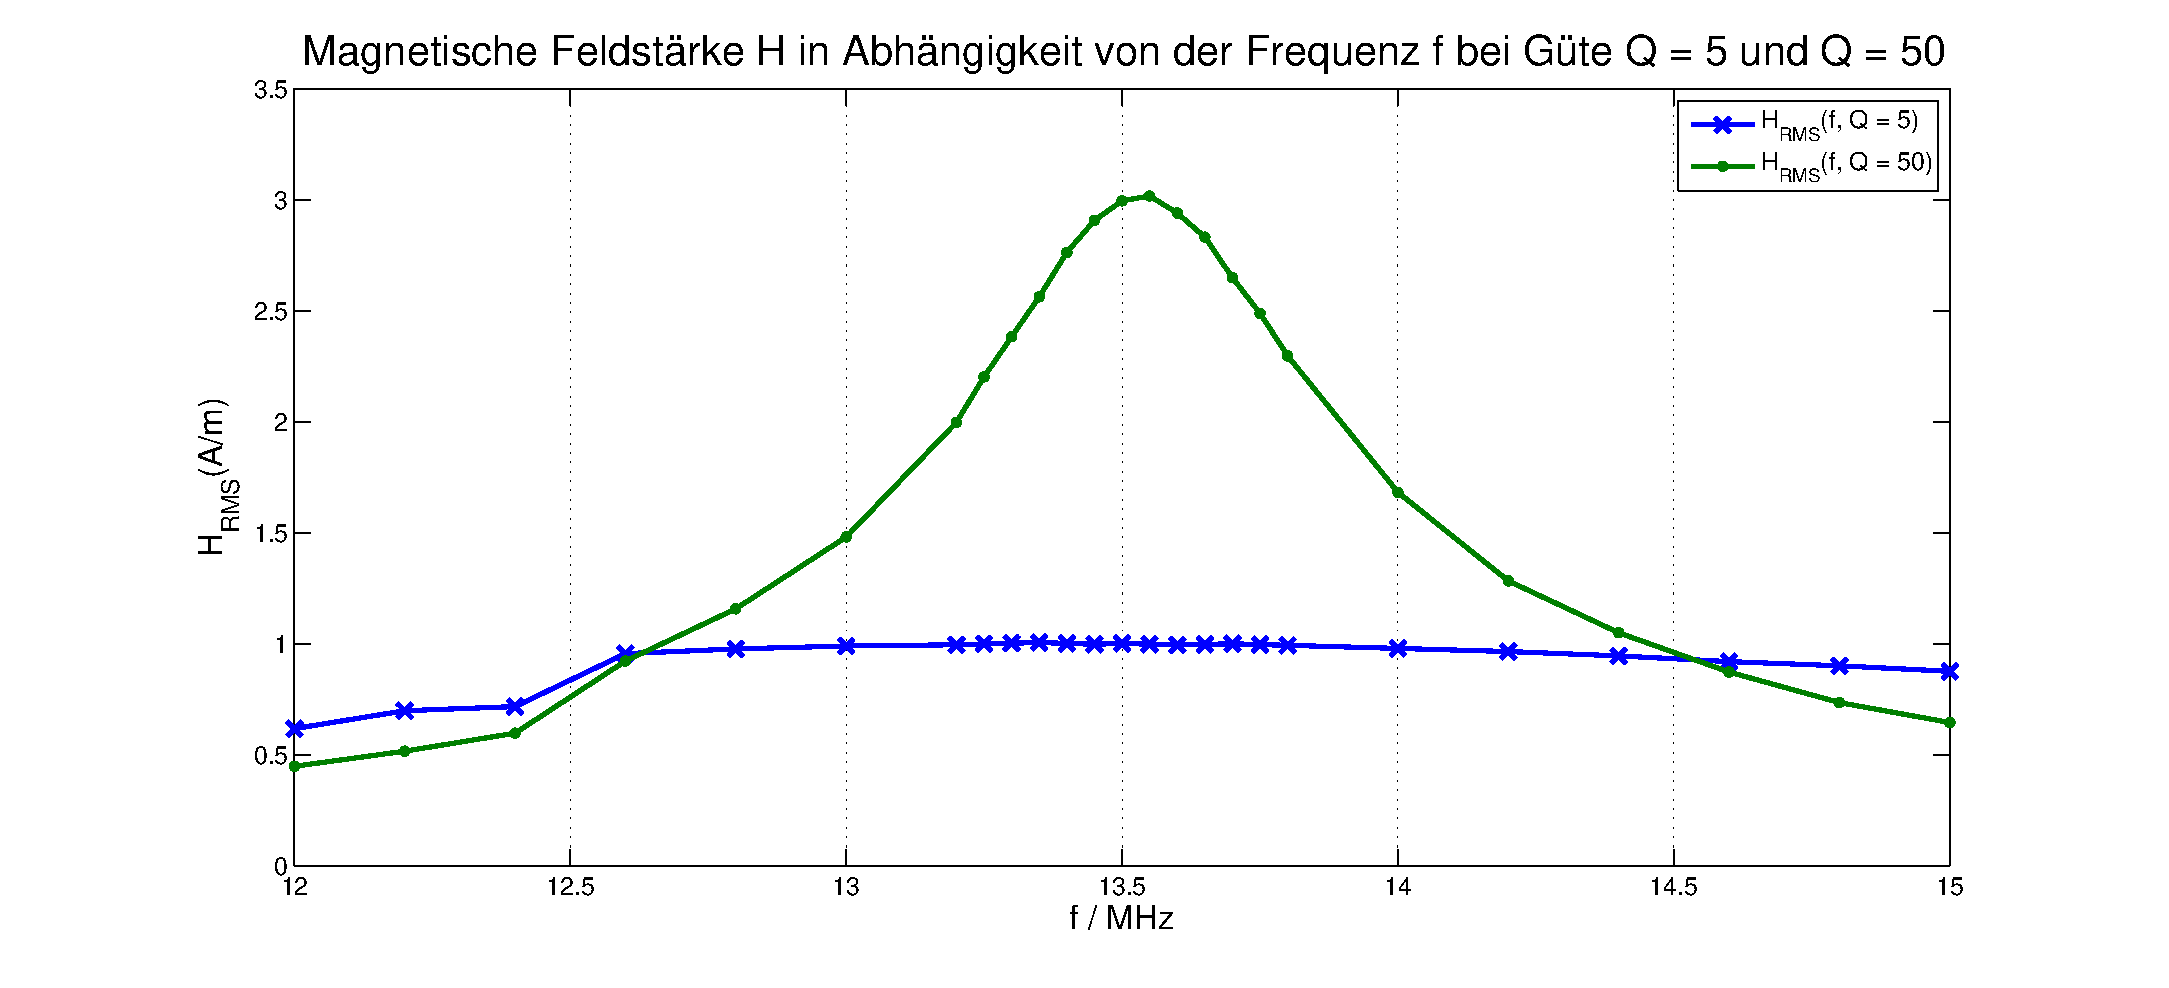
\includegraphics[width=0.9\textwidth]{figures/a2.eps} 
\caption{Frequenzgang beider Antennen}\label{fig:a2}
\end{figure}

\subsection{Geräteliste}
\begin{itemize}
\item Funktionsgenerator: LeCroy LW120
\item Verstärker: Amplifier Research Model 75A250
\item Dämpfer: 6dB
\item Antennen: PCD-Schleifenantennen mit Q=5 und Q=50
\item Referenzspule mit Abmessungen 72mm x 42mm
\item Oszilloskop: Agilent 54622D
\item ISO-Aufbau
\end{itemize}


\subsection{Diskussion}
Am Funktionsgenerator wurden 13.56MHz und eine Amplitude von 100mV eingestellt. Der Verstärker wurde so eingestellt, das am Oszilloskop $2.77$V Spitze-Spitze-Spannung abzulesen waren. 
Dies entspricht einer Feldstärke von $3 \frac{\text{A}}{\text{m}}$. \\
Während der Messung wurde der Frequenzgenerator von 12-15MHz in 200kHz Schritten verstellt und dabei die Spitze-Spitze-Spannung am Oszilloskop abgelesen. Um die Resonanzfrequenz wurden mehrere Werte in einem engeren Abstand von 50kHz abgelesen (13.2-13.8MHz).
Diese Messung wurde für beide Antennen durchgeführt. \\
Für die Antenne mit der Güte 50 erkennt man rund um die Resonanzfrequenz einen starken Anstieg der magnetischen Feldstärke und genau auf der Resonanzfrequenz den Maximalwert von $3.025\frac{\text{A}}{\text{m}}$. Für die Antenne mit der Güte 5 sieht man einen flacheren Verlauf der Kurve, der Maximalwert liegt bei $0.982\frac{\text{A}}{\text{m}}$. Dieser ist allerdings bei 13.56 MHz zu finden, sondern bei 13.95MHz, da die Antenne in dem Aufbau leicht verstimmt war. Außerdem war zu sehen, das die Antenne mit niedrigerer Güte bei gleichem Aufbau und Verstärkung nur mehr $\frac{1}{3}$ der Feldstärke erzeugt. \\
Aus Abbildunng (\ref{fig:a2}) erkennt man, das bei niedrigen sowie hohen Frequenzen die Antenne mit höhere Güte eine höhere Dämpfung aufweist. 
\pagebreak



\section{Arbeitsbereich eines Lesegerätes}
\subsection{Aufgabenstellung}
Bei dieser Aufgabenstellung soll Referenz-PICC vermessen werden (Ausgegebene Gleichspannung bei gegebener Feldstärke). Weiters soll überprüft werden, ob eine gegebene Karte ISO-konform ist. 
\subsection{Messaufbau}
Die Antenne mit Güte 50 wurde über den Dämpfer und den Verstärker am Funktionsgenerator angeschlossen und in den ISO-Aufbau mittig eingebracht. Auf der einen Seite des ISO-Aufbaus wurde die Referenz-Spule und auf der anderen Seite der Referenz-PICC befestigt. Die Spannung der Referenz-Spule wurde mit dem Oszilloskop und die Gleichspannung am Referenz-PICC mit dem Multimeter gemessen. \\
Im zweiten Teil der Unterübung wurde statt dem ISO-Aufbau der Distanzhalter und statt dem Funktionsgenerator der RFID-Reader verwendet. 

\subsection{Tabellen}
\begin{table}[H]
\begin{center}
\begin{tabular}{ |c|c|c| }
  \hline

    H(rms)) & $U_i(pp)\ am\ Scope$ & $U_i(pp)\ am\ Transponder$\\

	{[A/m]} & {[V]} & {[V]} \\
  \hline
  0 & $0$ & $0$\\
  \hline
  $0.498$ & $0.456$ & $0.982$ \\
  \hline
  $0.997$ & $0.913$ & $1.933$\\
  \hline
  $1.4677$ & $1.344$ & $3.154$\\
    \hline
  $1.9656$ & $1.8$ & $4.21$\\
    \hline
  $2.4352$ & $2.23$ & $5.26$ \\
    \hline
  $2.9375$ & $2.69$ & $6.29$\\
     \hline
  $3.4835$ & $3.19$ & $7.46$ \\ 
    \hline
  $3.9421$ & $3.61$ & $8.5$  \\
    \hline
  $4.4663$ & $4.09$ & $9.5$  \\
    \hline
  $5.0123$ & $4.59$ & $10.52$  \\
    \hline
  $5.4928$ & $5.03$ & $11.55$  \\
    \hline
  $5.9733$ & $5.47$ & $12.55$ \\
     \hline
  $6.4537$ & $5.91$ & $13.53$ \\
      \hline
  $6.9233$ & $6.34$ & $14.55$ \\ 
      \hline
  $7.4038$ & $6.78$ & $15.56$  \\
      \hline
  $7.8515$ & $7.19$ & $16.5$  \\
      \hline 
\end{tabular}
\caption{Gleichspannung am PICC in Abhängigkeit der magnetischen Feldstärke}
\label{tab:3}
\end{center}
\end{table} 

\subsection{Formeln}
Diese Formel stellt den Zusammenhang zwischen induzierter Spannung und Feldstärke dar. Die verwendeten Parameter sind $f_r = 13.56$MHz, $\mu_0 = 4\pi \cdot 10^{-7}\frac{As}{Vm}$, $\mu_r = 1$ und $A = 0.072 \cdot 0.042\ m^2$.
\begin{equation}
U_{ind} = 2\pi \cdot f_r \cdot \mu_0 \cdot \mu_r \cdot H \cdot A
\end{equation}

Zusammenhang zwischen Spitze-Spitze-Spannung und dem Effektivwert der Spannung.
\begin{equation}
U_{pp} = \sqrt{2}  \cdot 2 \cdot U_{ind}
\end{equation}
\subsection{Berechnungsbeispiele}
Die Werte für das Berechnungsbeispiel wurden aus der Tabelle \ref{tab:3} Zeile 2 entnommen.
\begin{equation}
U_{ind} = \frac{U_{pp}}{\sqrt{2}  \cdot 2} = \frac{0.456V}{\sqrt{2}  \cdot 2} = 0.161 V
\end{equation}

\begin{gather}
H = \frac{U_{ind}}{2\pi \cdot f_r \cdot \mu_e \cdot \mu_r \cdot A} = \\
\frac{0.161V}{2\pi \cdot 13.56MHz \cdot 4\pi \cdot 10^{-7}\frac{As}{Vm} \cdot 1 \cdot 0,072m \cdot 0,042m} = 0.498\frac{A}{m}
\end{gather}

\pagebreak
\subsection{Diagramme}
\begin{figure}[H]
\centering
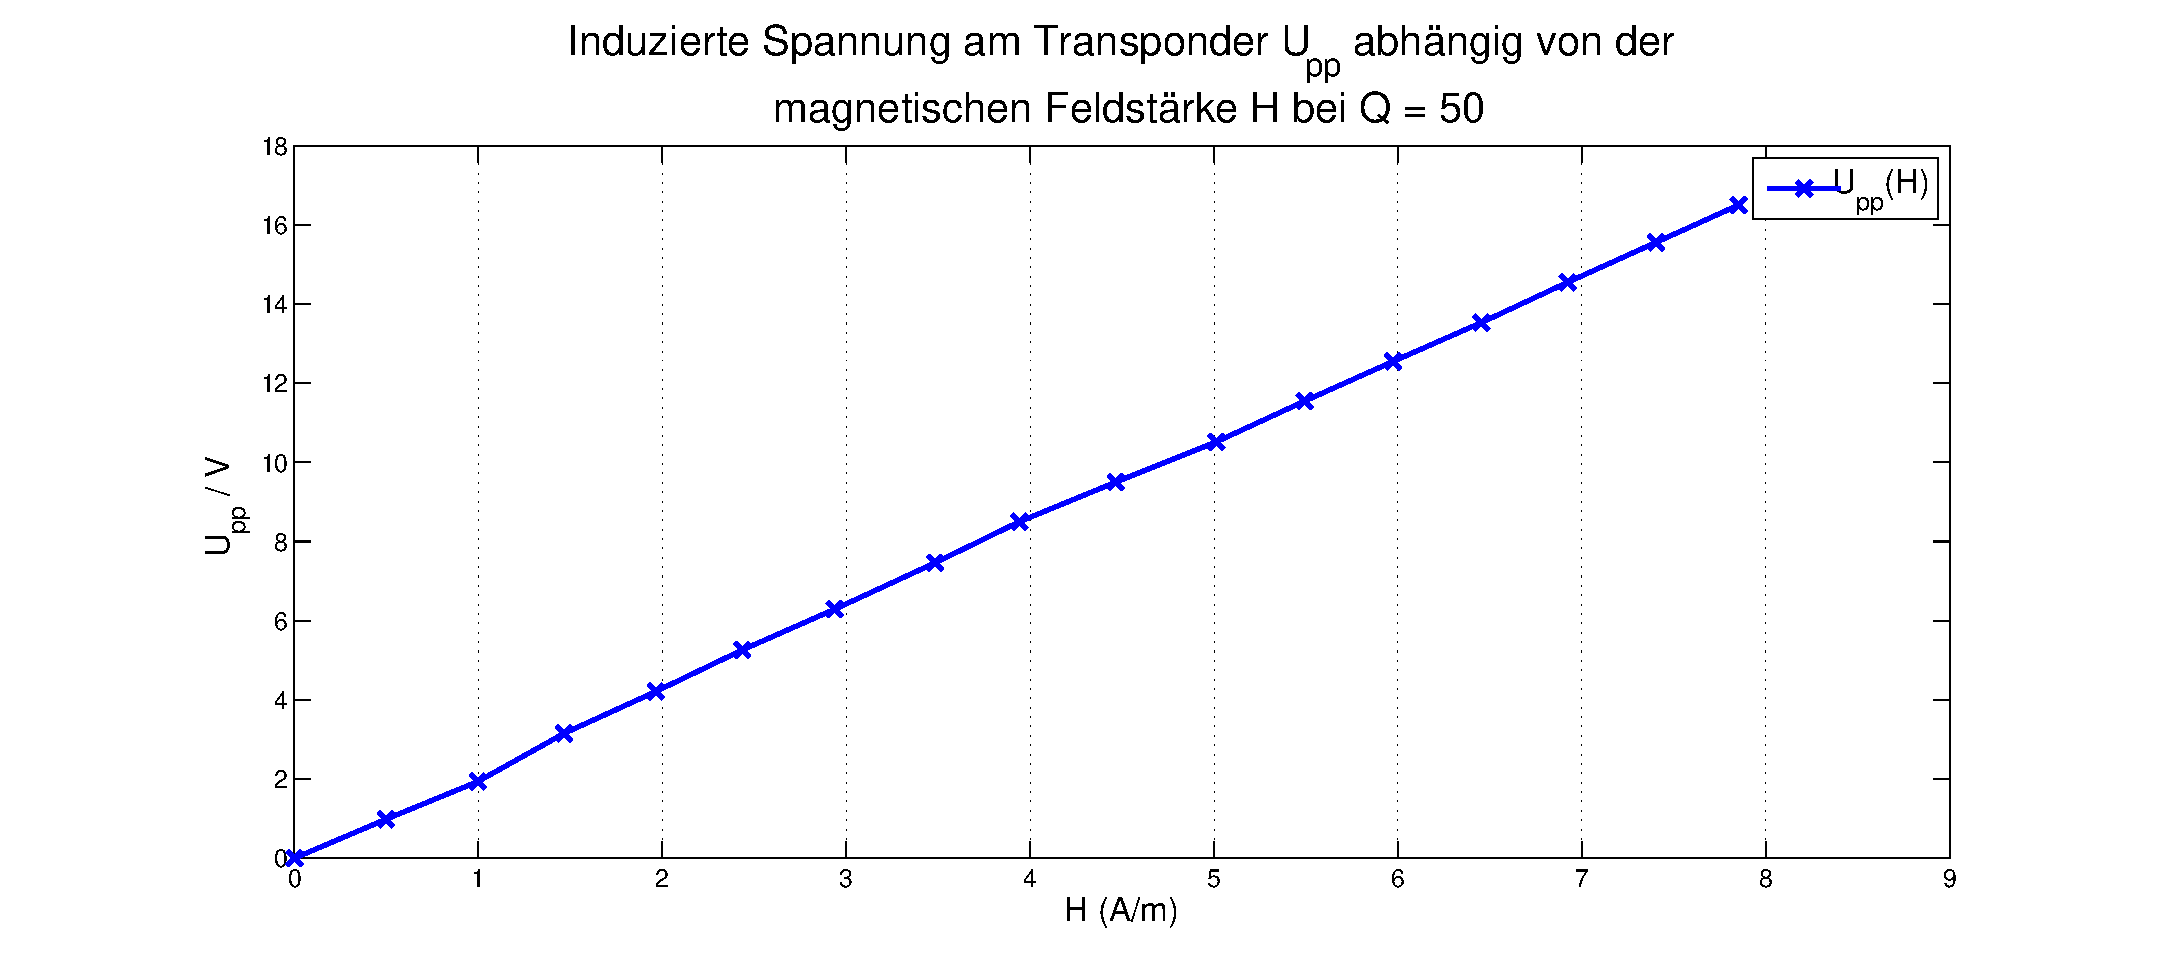
\includegraphics[width=0.9\textwidth]{figures/a3.eps} 
\caption{Verlauf der Spannung am Transponder bei verschiedenen magnetischen Feldstärken, bei einer Antennengüte von Q=50}
\label{fig:3}
\end{figure}

\subsection{Diskussion}
Am Beginn dieser Aufgabe wurde der Funktionsgenerator auf 13.56MHz und eine Amplitude von 100mV eingestellt. 
Die Verstärkung wurde so eingestellt, sodass an der Referenz-Spule 0.913V (1$\frac{\text{A}}{\text{m}}$) gemessen werden.
Danach wurde die Amplitude des Funktionsgenerators in $50 \text{mV}$ (entspricht $0.5 \frac{\text{A}}{\text{m}}$) Schritten erhöht und die Spannung am Referenz-PICC gemessen. \\
Wie aus Abbildung (\ref{fig:3}) ersichtlich, steigt die Spannung am Referenz-PICC linear mit der magnetischen Feldstärke. \\
Im zweiten Teil der Unterübung wurde der ISO-Aufbau mit dem Distanzhalter und der Funktionsgenerator mit dem (Mifare NXP)-Reader ersetzt. 
Der Abstand zwischen Reader und Referenz-PICC wurde solange verändert, bis man den Abstand bei ISO-konformen Wert von $1.5\frac{A}{m}$($0.982$V am PICC) ermittelt hat. Da dieser Abstand größer als die von der ISO-Norm geforderte Distanz war, ist der Reader ISO-Konform. \\ Weiters wurde statt dem Referenz-PICC ein Transponder (Karte) verwendet. Am PC wurde bei gesendetem Lesebefehl die ID des Transponders angezeigt.  \\ 
Die maximale Funktionsweite der Lesegerät-Transponder-Kombination wurde mit 12 cm bestimmt.
Dies ist möglich, da die Karte weniger als $1.5\frac{A}{m}$ zum Betrieb benötigt. Somit erfüllt auch die Karte die ISO-Norm deutlich. 


\pagebreak
\section{Seitenbandpegel der Rückmodulation}
\subsection{Aufgabenstellung}
Bei dieser Aufgabe galt es die Amplituden der beiden Seitenbänder der Rückmodulation vom Transponder zu ermitteln. Hierfür soll die Helmholz-Anordnung verwendet werden. Mit Hilfe des Verstärkers soll die magnetische Feldstärke am Transponder von 1-6 A/m eingestellt werden. Danach soll eine ISO 14443 Karte in das Feld gebracht und ein Kommando über die PC-Software geschickt werden. Mit Hilfe der Helmholtz-Anordnung wird die Transponder-Antwort mit dem Oszilloskop aufgenommen. Die Amplituden der Seitenbänder werden mit Hilfe eines Oszilloskop-Screenshots und einer FFT-Software berechnet. 

\subsection{Messaufbau}

\begin{figure}[H]
\centering
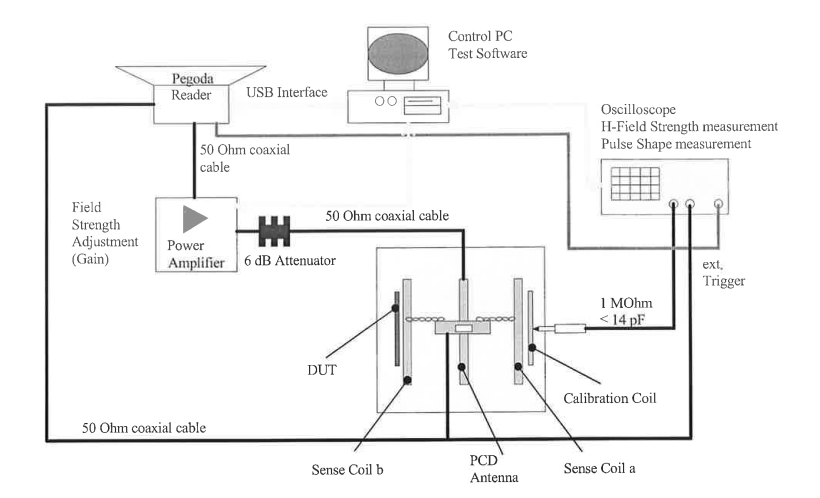
\includegraphics[width=0.9\textwidth]{figures/aufbau4.png} 
\caption{Messaufbau zu Aufgabe 4, entnommen aus Skript \cite[S.39 Abbildung 42]{skript}}
\label{fig:aufbau4}
\end{figure}

\subsection{Tabellen}

\begin{table}[H]
\begin{center}
\begin{tabular}{ |c|c|c|c| }
  \hline
    $U_{pp}$ & H(rms) & $U_i(pp)$ oberes Seitenband & $U_i(pp)$ unteres Seitenband \\
	 {[V]} & {[A/m]} & {[mV]} & {[mV]} \\
  \hline
  $0.913$ & $0.997$ & $320.6$ & $41.95$\\
  \hline
  $1.83$ & $1.9984$ & $866.21$ & $727.24$ \\
  \hline
  $2.75$ & $3.003$ & $158.54$ & $32.35$\\
  \hline
  $3.69$ & $4.0295$ & $218.7$ & $312.14$\\
    \hline
  $4.59$ & $5.0123$ & $175.37$ & $61.54$\\
    \hline
  $5.53$ & $6.0388$ & $323.9$ & $267.93$ \\
    \hline 
\end{tabular}
\caption{Amplitudenwerte der Seitenbänder bei verschiedenen magnetischen Feldstärken}
\label{tab:ue4}
\end{center}
\end{table} 

\subsection{Formeln}
Diese Formel stellt den Zusammenhang zwischen induzierter Spannung und Feldstärke dar. Die verwendeten Parameter sind $f_r = 13.56$MHz, $\mu_0 = 4\pi \cdot 10^{-7}\frac{As}{Vm}$, $\mu_r = 1$ und $A = 0.072 \cdot 0.042\ mm^2$.
\begin{equation}
U_{ind} = 2\pi \cdot f_r \cdot \mu_0 \cdot \mu_r \cdot H \cdot A
\end{equation}

Zusammenhang zwischen Spitze-Spitze-Spannung und dem Effektivwert der Spannung.
\begin{equation}
U_{pp} = \sqrt{2}  \cdot 2 \cdot U_{ind}
\end{equation}

\subsection{Berechnungsbeispiele}
Die Werte für das Berechnungsbeispiel wurden aus der Tabelle (\ref{tab:ue4}) Zeile 1 entnommen.
\begin{equation}
U_{ind} = \frac{U_{pp}}{\sqrt{2}  \cdot 2} = \frac{0.913V}{\sqrt{2}  \cdot 2} = 0.323V
\end{equation}

\begin{gather}
H = \frac{U_{ind}}{2\pi \cdot f_r \cdot \mu_e \cdot \mu_r \cdot A} = \\
\frac{0.323V}{2\pi \cdot 13.56MHz \cdot 4\pi \cdot 10^{-7}\frac{As}{Vm} \cdot 1 \cdot 0.072mm \cdot 0.042mm} = 0.997 \frac{A}{m}
\end{gather}

\subsection{Diagramme}
\begin{figure}[H]
\centering
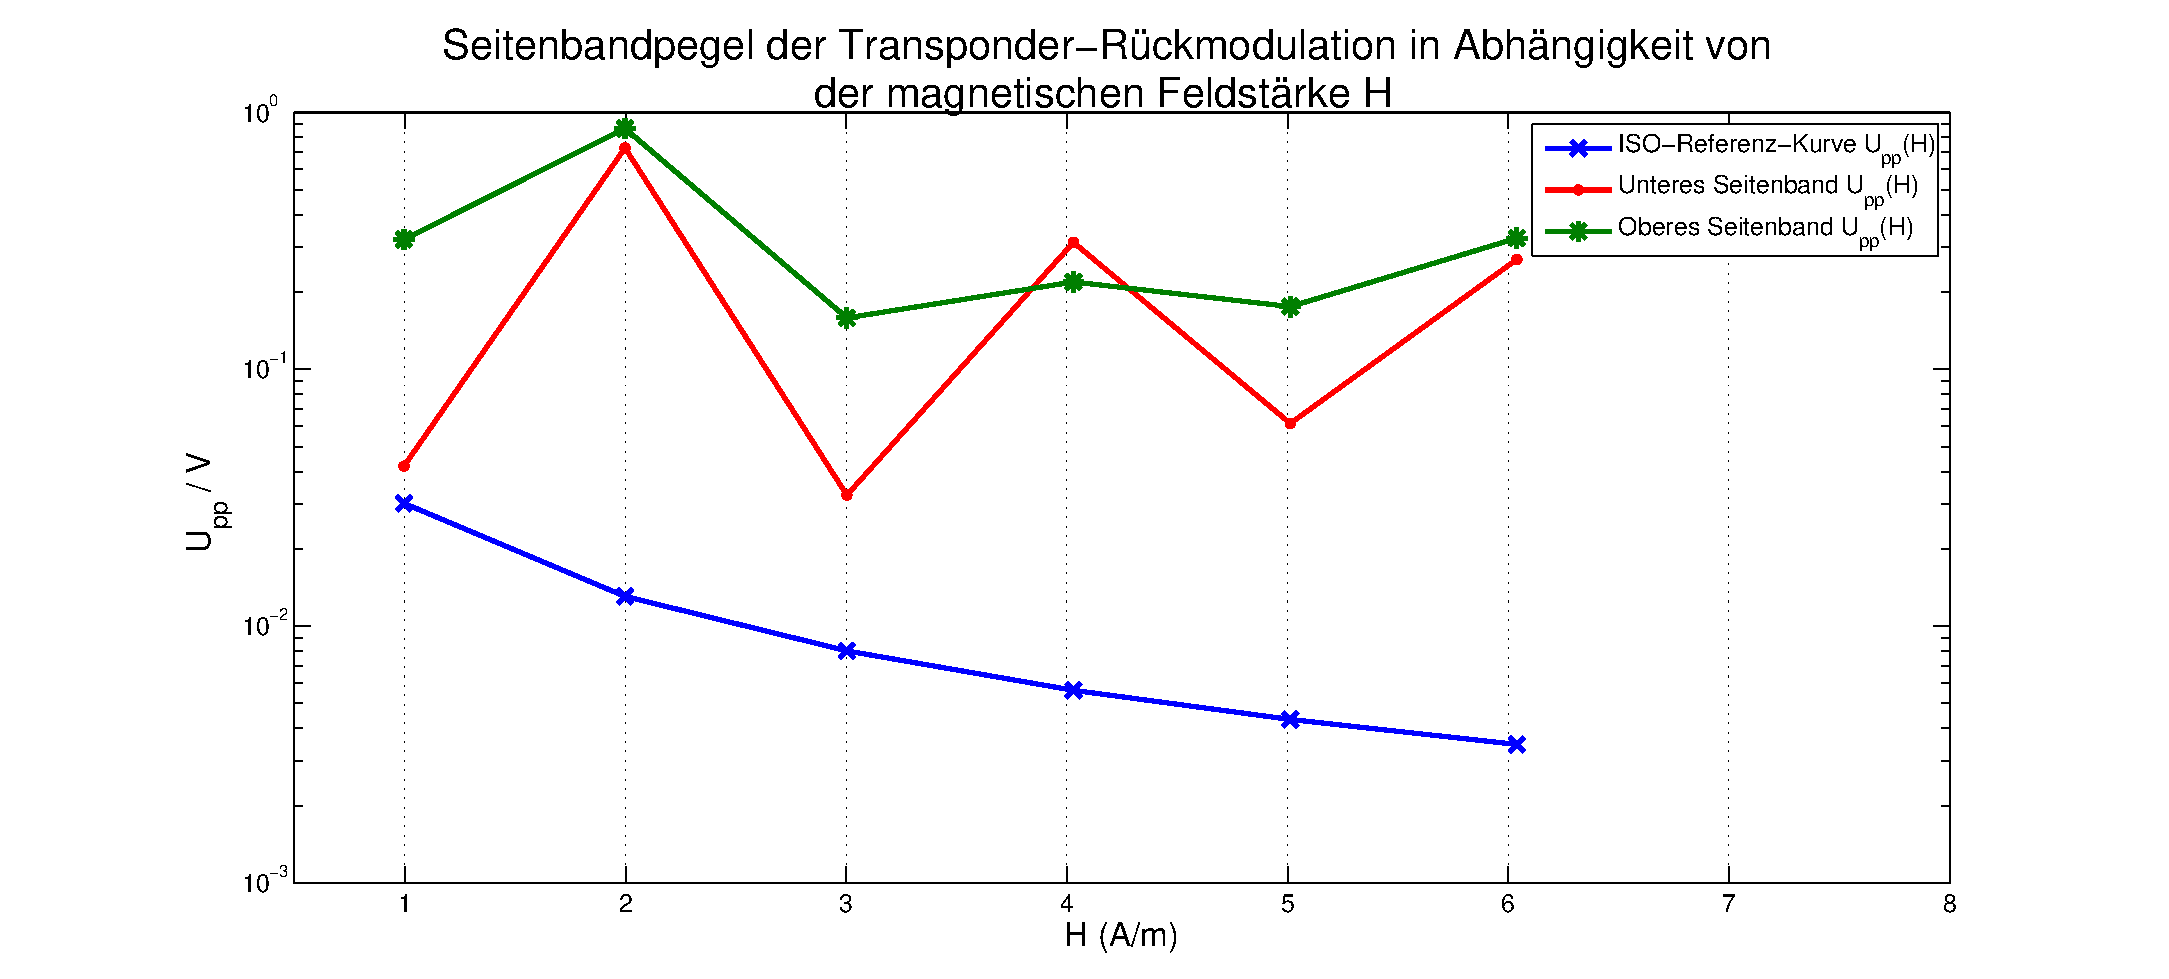
\includegraphics[width=0.9\textwidth]{figures/a4.eps} 
\caption{Seitenbandpegel bei verschiedenen Feldstärken im Vergleich zur ISO-Norm-Kurve}
\label{fig:a4}
\end{figure}

\subsection{Diskussion}
Um die Amplituden der Seitenbänder zu ermitteln wurde mit Hilfe des Oszilloskopes ein Single-Shot der Antwort der Karte aufgenommen. Dieses Ergebnis wurde als CSV auf eine Diskette gespeichert und am Computer wurde, mit Hilfe einer speziellen Software, daraus die FFT berechnet. Als Ergebnis haben wir die Amplitudenwerte des oberen und unteren Seitenbandes bekommen. Diese können aus Tabelle (\ref{tab:ue4}) entnommen werden. In Abbildung (\ref{fig:aufbau4}) wurden die beiden Seitenbänder über der magnetischen Feldstärke aufgetragen. Außerdem wurde der ISO-Grenzwert ($U_i(pp)\geq\frac{30}{H^{1.2}}$)mit eingetragen. Wie aus der Abbildung entnommen werden kann, befinden sich beide Seitenbänder über dem von der ISO-Norm geforderten Wert.


\begin{thebibliography}{9}

\bibitem{skript}
  Teresa Meier, Dipl.-Ing. Georg Egger, Dipl.-Ing. Dr Michael Gebhart\\
  \emph{Übung C: RFID}\\
  Technische Universität Graz
\end{thebibliography}

 



   
\end{document}
